
\section{Introduction}

The goal of exploration seismology is to find oil and gas reservoirs
by seismically imaging the earth's reflectivity distribution. Towards
this goal, exploration geophysicists perform seismic experiments ideally
equivalent to that shown in Figure (\ref{fig:oil-drilling}).

\begin{figure}[h]
\centering
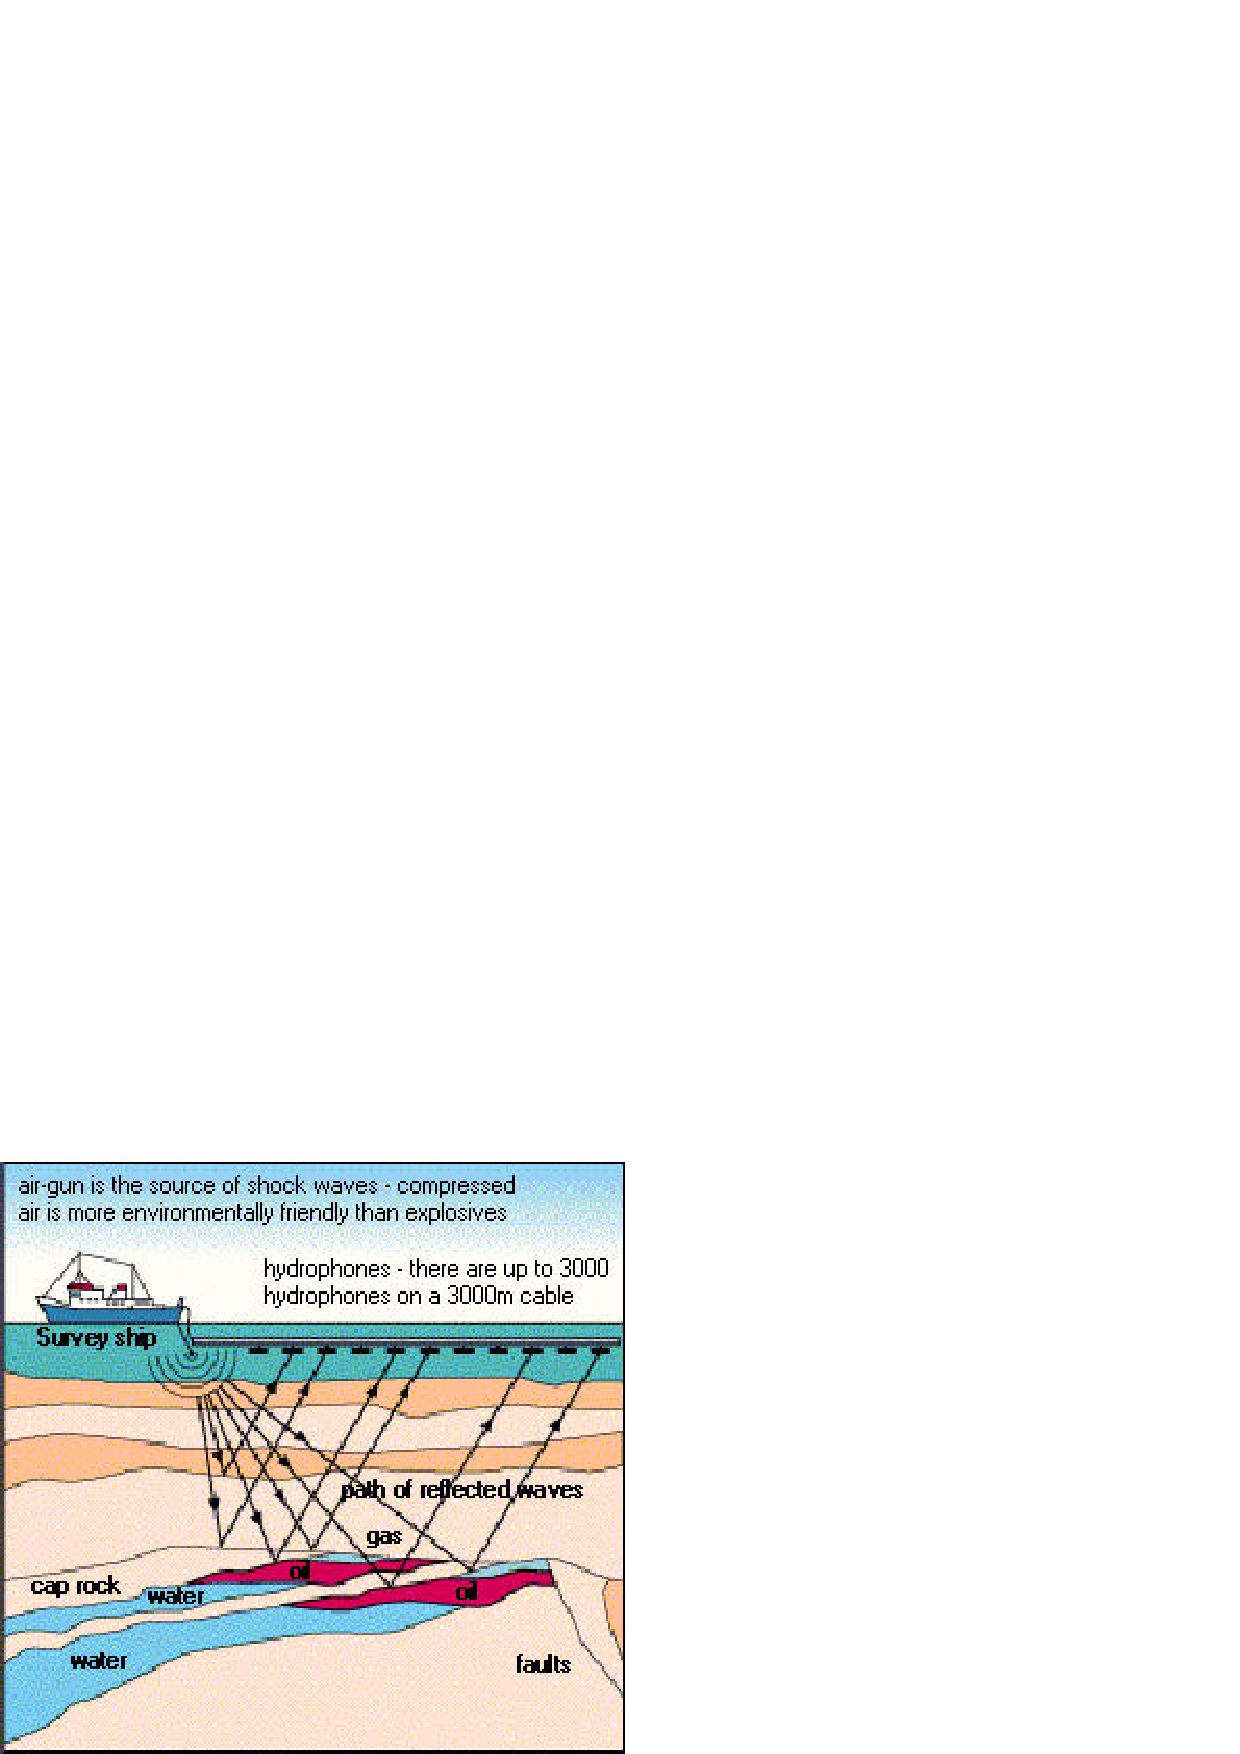
\includegraphics[scale=0.65]{img/oil-drilling-prospecting2.jpg}
\caption{Searching for oil over water using seismology}
\label{fig:oil-drilling}
\end{figure}

Here,
the survey ship excites seismic waves by its air gun, and the resulting
primary reflections are recorded by a set of hydrophones. The geologists
are the ones responsible for finding the oil trap or gas trap by processing
and analyzing the 3D wave fields that are reflected back by the subsurface.
However, only with the help of computers and engineers could the data
be processed and analyzed because terabytes of data would be processed.
The computational performance plays an important role through out
the process because the Reverse Time Migration (RTM) algorithm is
a high computational-demanding imaging algorithm.%
\footnote{The complexity of RTM for a single shot is roughly \BigO{n4}%
}



The ultimate and perhaps unattainable goal of computer science is
to make the computer to do whatever we want in perfect accuracy, speed,
security and on and on. Over time, the number of transistor on integrated
circuit doubles approximately every two year, which greatly improves
the computational performance and memory capacity of the general purpose
computer. However, as CPU speeds and memory capabilities have increased,
other aspects of performance, such as the access speed of register
and memory, or the access speed of memory and disk, have failed to
keep up. As a result, the performance of the whole system isn't likely
to improve a lot, and the access latencies frequently become a bottleneck
in the system.

Lots of efforts have been made facing with the access latencies, and
some of the methods gained extraordinary achievement. For example,
the vendors who manufacturing the chips try to use \emph {out-of-order
execution}  paradigm to make use of instruction cycles that would
be otherwise be wasted by a certain type of costly delay. One more
well-known ways to reduce the latencies between the fast-speed CPU
registers and relative-low-speed main memory is use \emph {caching.}
By storing the copy of data that are frequently accessed by the
processor into the cache, the amount of time that processors read
and write directly from/to memory decrease significantly, thus improves
the overall performance.

Such kinds of techniques, out-of-order execution, on-chip cache and
prefetching that we didn't mention before, does reduce the memory
latencies bottleneck, however, it also requires more transistors for
designing the processors, and the design of processors becomes more
and more complicated. What's worse, when the consecutive read/write
instructions cover a wide range of memory location, or the memory
access pattern is too random to predict, the application will suffer
from a high ratio of cache misses and the memory bottleneck re-emerge\cite{fu11}.

The current trend of improving the computer performance can be divided
into three category, increase the clock rate, fitting more and more
cores into a single processor, multiple computers (nodes) cooperate
together, and use some co-processors.

For years, processor makers consistently delivered increases in clock
rates and instruction-level parallelism, so that single-threaded code
executed faster on newer processors with no modification\cite{herb11}.
However, For a given device, operating at a higher clock rate always
requires more power. Especially, the high clock rate cannot be tolerated
in cluster computing or grid computing, or super computing, because
there are hundreds of thousands of processors within a cluster. That
is why the clock rate of servers servers generally stays between 2.0Ghz
and 2.4Ghz.

Now, to manage the CPU power dissipation, processor makers favor multi-core
designs, that is, integrate more than one core into a single processor,
such as the Intel Ferry CPUs, which have up to 32 cores. Following
the change of the CPU architecture, the software has also to be changed
at the same time. The previously single-thread (single-process) programs
have to be modified to multi-thread (multi-process) manner to take
full advantage of the hardware. Most of the multi-threaded development
paradigms introduce new overhead, and you will not see a linear increase
in speed vs number of processors. This is particularly true while
accessing shared or dependent resources, due to lock contention. This
effect becomes more noticeable as the number of processors increases\cite{moore}.

The computational performance for a single computer (node) is not
enough to support most of the science computation. Generally, scientists
and some of the industries would set up a \emph{cluster}, which consists
of a set of loosely connected or tightly connected computers that
work together so that in many respects they can be viewed as a single
system. Compared with a personal computer, the whole cluster certainly
has higher performance, but it also costs more power and the average
performance of a single node of the cluster is much lower than that
works individually. The entire performance of the cluster may even
increase slower when the number of nodes increase. What's more, for
a cluster, more aspects should be taken into consideration for tunning
the performance, including networking bandwidth and latency, parallel
file system performance, the application scalability and so on.

The most powerful supercomputer \emph{Titan}, which is made by Cray
Inc, has 560640 cores, 710144GB memory and it reaches high a Linpack
Performance of 17590.0 TFlops\footnote {Flops: number of double-precision
floating point operation per second} with its power being 8209kw\cite{top500}.
The scientist yet seems not content with the current computational
power because even by using the super computer, it still takes several
months or even several years to run some of simulation, such as seismic
imaging, weather simulation, ocean simulation, or global simulation.
And they need higher computational performance for a higher resolution
of the simulation.

Some vendors manufacture co-processor to aid CPU to better perform
general computing. For example, the NVIDIA Cooperation publish its
GPU accelerating card, which consists of hundreds of core in a single
card \footnote{There are 512 cores in NVIDIA Fermi GPUs}. GPU is better at general arithmetic
computation than general purpose CPU not only because it has more
cores than CPU, but also because its ratio of FLOPS  to power is much
higher than CPU. It can save lots of power in a cluster. The NVIDIA Inc
provides a set of
API, eg. CUDA C, for programmer to develop applications running on
NVIDIA card. The programs running on GPU cards are similar to the
programs running to CPU. In a word, they are both software.

Some vendors and researches still trying to increase the computational
performance as well as the ratio of FLOPS to power. You may wonder
whether we can build our application in hardware level instead of
software level, which could satisfy the vendors and researchers' willing.
That is why FPGA emerged.

A \emph {field-programmable gate array} (FPGA) is an integrated
circuit that is designed to be configured by the customer or a designer
after manufacturing, thereby \emph {field-programmable.}

The magic of FPGAs is that the connections among the logic gates (the
actual circuit you need) are made at power-up by reading the configuration
instructions written into a bit file. Changing the file changes the
function of the FPGA.

In this paper, I present my FPGA-based solution for the Reverse Time
Migration (RTM) algorithm ~\cite{yoon03}, which is the most computationally-demanding
imaging algorithms in oil and gas exploration.

The Reverse Time Migration (RTM) is a wave equation depth migration
method. It offers insights into geology that were previously impossible
to interpret or understand using seismic data.

Conventional migration methods, generally, use standard wave equation
techniques with mathematical approximations assuming that wave field
propagate in only one field. RTM is a two-way migration solution that
more accurately implements the wave equation and provides an alternative
approach to migration with fewer compromises. RTM works by running
the wave equation forward in time for the source and backwards in
time for the receiver ~\cite{shafiq}.

The RTM algorithm generally needs to deal with source and receiver
3D wave field arrays at thousands of different time steps, which brings
the requirement to manipulate terabytes of data in disk or in memory.
The kernel of the RTM algorithm, which applies a large 3D stencil
over a 3D data cube, needs to access a wide range of memory locations
while computing the result of one point. In many cases, the computation
incurs a large number of cache misses and reduces the performance
significantly. These highly demanding memory access characteristics
of RTM form a 'memory wall' that keeps us from achieving high throughput
in common computer clusters ~\cite{fu11}.

In this work, by utilizing the great computing performance of FPGA
and enormous internal memory bandwidth of the FPGA, I manage to implement
the computationally-demanding Reverse Time Migration algorithm in
FPGA.
